\section{Case Studies}
\label{sec:case-studies}

Here we examine three case studies involving elliptic \gls{pdes}. For all iterative methods, the relative tolerance is set to $\tau_{\text{rel}} = 1 \times 10^{-12}$ and the maximum number of iterations allowed is $N_{I,\textsc{max}} = 10000$. For all cases, the effective resolution, which is the resolution of the domain at the finest level if the mesh is adaptive, will vary from $R_{\text{eff}} = [128, 256, 512, 1024, 2048]$. All runs were done in parallel on a 2021 MacBook Pro (M1 Pro CPU with 8 cores, 32GB RAM).

\subsection{Case 1: The Poisson Equation}
\label{sub:case01}

The first case study solves
\begin{align}
    \nabla^2 u(x,y) = -2(y^2 - y^4 + x^4(6y^2 - 1) + x^2 (1 - 12y^2 + 6^4))
\end{align}
for $(x,y) \in \Omega = [-1,1]^2$, which has the exact solution
\begin{align}
    u(x,y) = x^2 (1 - x^2) y^2 (y^2 - 1).
\end{align}
Dirichlet boundary conditions are supplied at the boundary using the exact solution. This problem is chosen to allow for refinement at the corners for any solver that can take advantage of adaptivity.

For adaptive solvers, the mesh is refined according to the right-hand side, which represents the curvature of the solution and is a good first attempt at \gls{amr} for elliptic \gls{pdes}. The AMR refinement is kept at $L_{\text{min}} = 2$ to $L_{\text{max}} = 5$ and the refinement threshold is $\epsilon_R = 0.5$, while we vary the patch size as $M = [4, 8, 16, 32, 64]$ to produce higher effective resolution.

% \begin{landscape}
    \begin{figure}
        \centering
        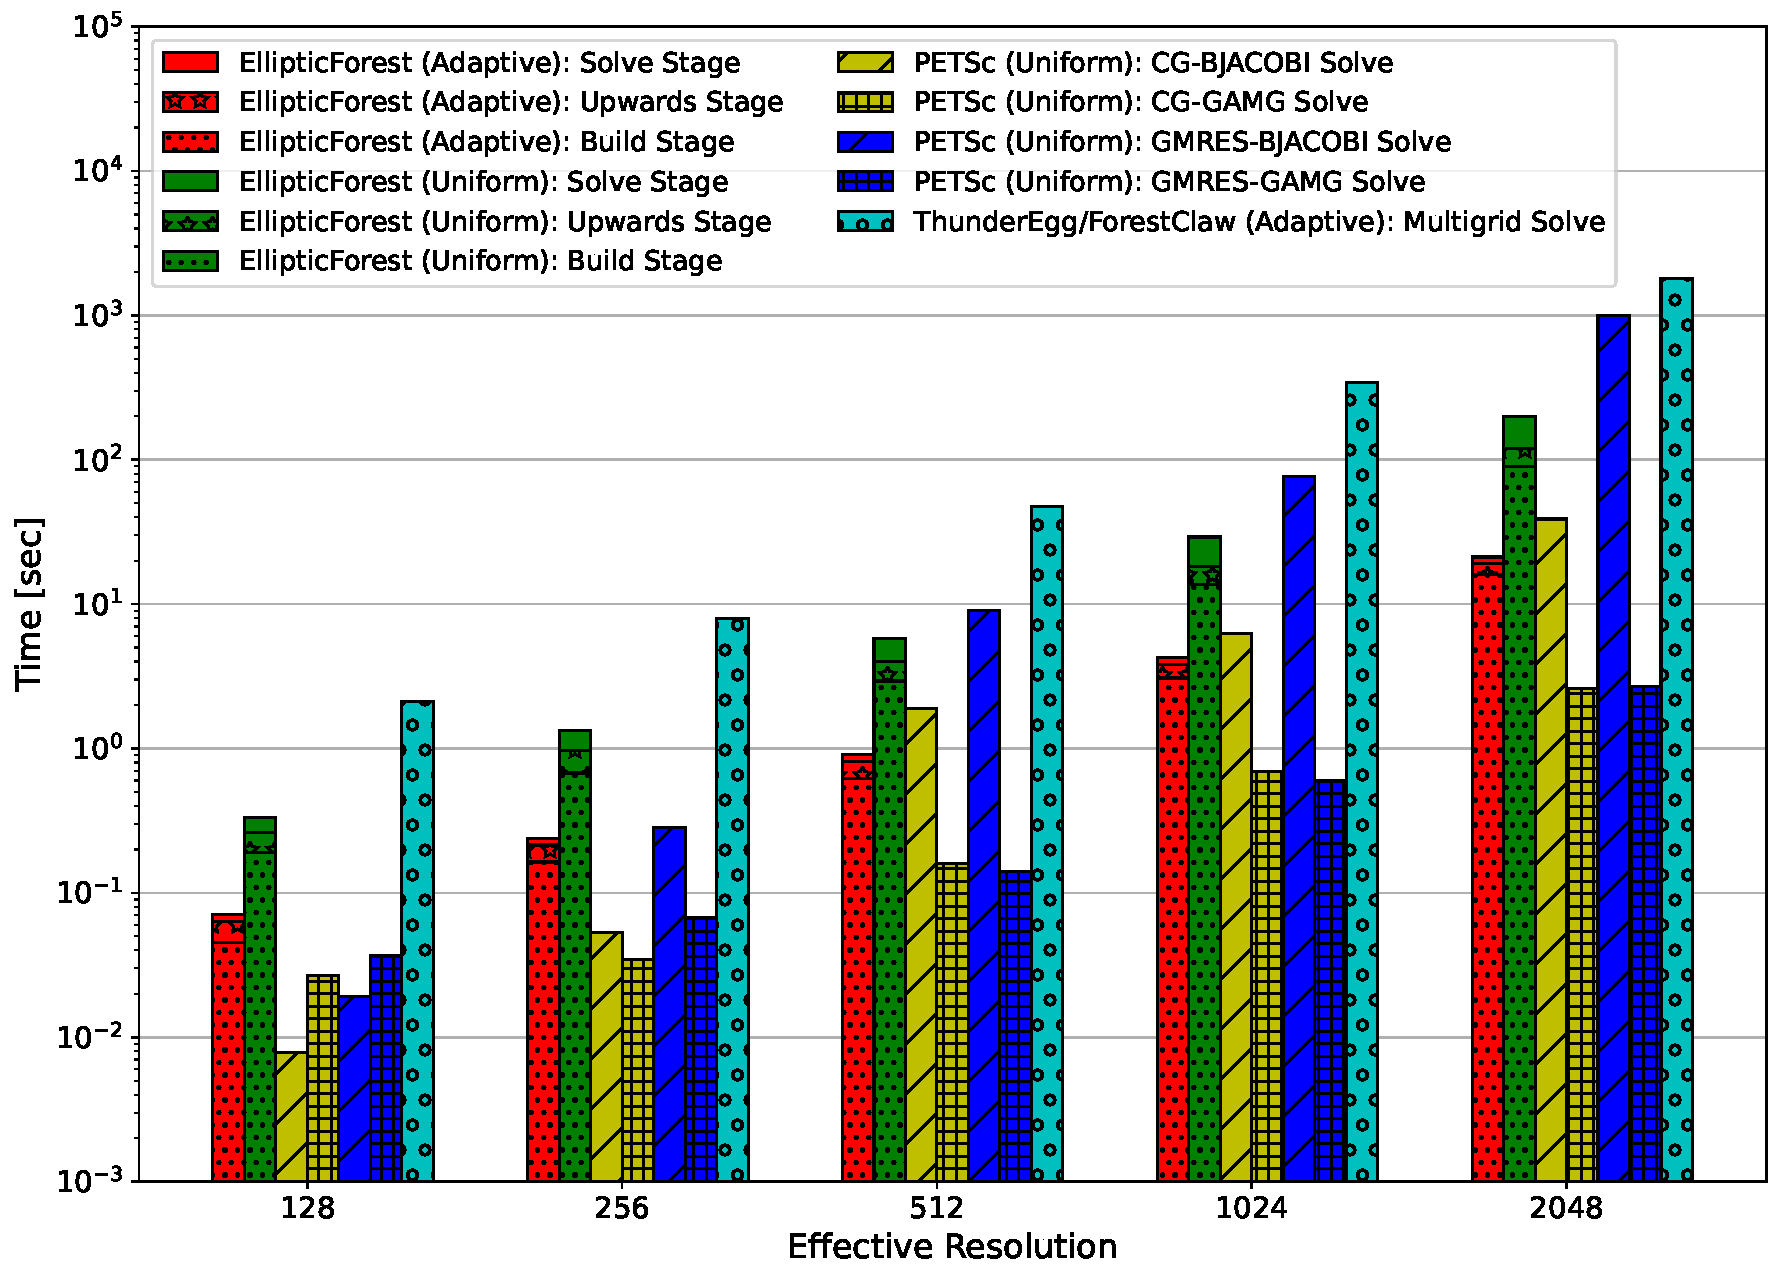
\includegraphics[width=1.0\textwidth, clip=true, trim={0 0 0 0}]{figures/case01-stacked-bar-plot-comparisons-no-title.pdf}
        \caption{Effective resolution vs. timing plot for Case 1 (\refsec{sub:case01}). The effective resolution is the number of cells per side if the mesh were refined to $L_{\text{max}}$. Each color indicates a different method/solver. Patterns indicate different stages or preconditioners. Lower is better.}
        \label{fig:case01-stacked-bar-plot}
    \end{figure}
% \end{landscape}

\begin{figure}
    \centering
    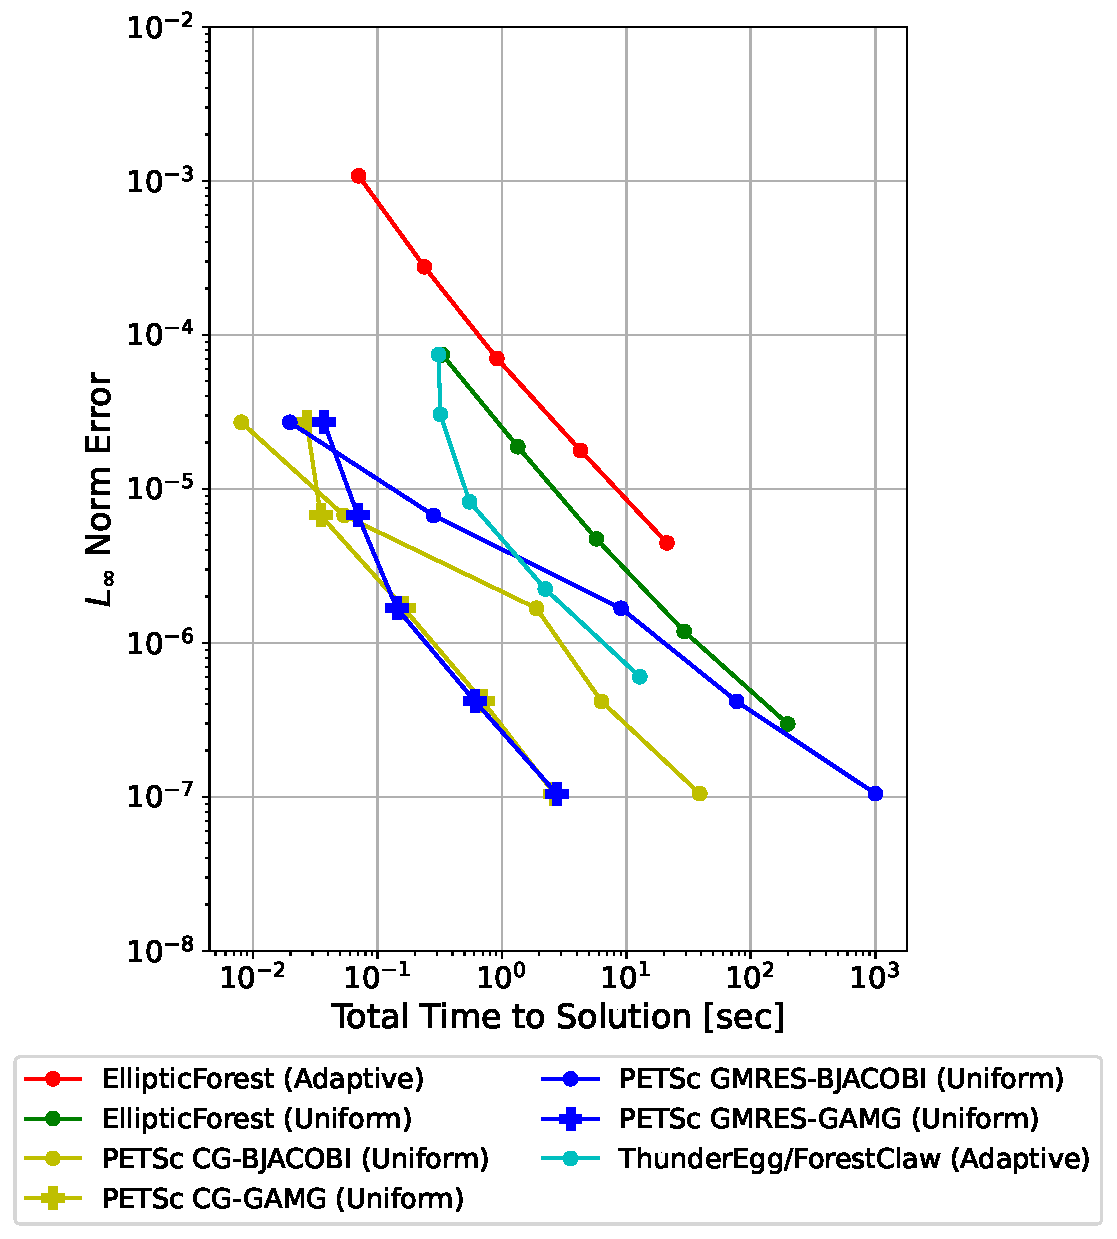
\includegraphics[width=1.0\textwidth, clip=true, trim={0 0 0 0}]{figures/case01-work-precision-plots-no-title.pdf}
    \caption{Work-precision plot for Case 1 (\refsec{sub:case01}). Colors indicate different methods and solvers, while markers indicate the type of preconditioner for certain iterative solvers. For work-precision plots, curves that lie in the lower-left portion of the plot are better.}
    \label{fig:case01-work-precision-plot}
\end{figure}

{\bf Discussion}
When using a five-point stencil approach to solve the Poisson equation, the resulting linear system is \gls{spd}. For the \gls{qahps} method, this means we can employ optimizations in the build stage such as operator caching (see \refrem{thm:operator-caching}) and when building the \gls{d2n} matrix (see \refsec{sub:building-leaf-level-operators}). As a constant coefficient elliptic \gls{pde}, we can use the FISHPACK patch solver, which is faster than the five-point stencil patch solver. For iterative methods, we can use the \gls{cg} method, which has accelerated convergence compared to general iterative solvers. For this case study, we show results with PETSc's \gls{cg} solver as well as \gls{gmres}, each with either a block Jacobi or \gls{amg} preconditioner. Timing results for increasing resolution is found in \reffig{fig:case01-stacked-bar-plot} and a work-precision plot is found in \reffig{fig:case01-work-precision-plot}.

The stacked bar plot in \reffig{fig:case01-stacked-bar-plot} shows timing results for increasing effective resolution. It shows how each code/method compares against each other in time to solution for the Poisson equation. For the \gls{qahps} methods (uniform and adaptive), the time to solution is partitioned into the build, upwards, and solve stages.

At the lower resolutions, PETSc's iterative solvers are very fast to converge. As the effective resolution increases, the time to solution for the block Jacobi preconditioners rapidly increases, while the \gls{amg} preconditioned solvers scale better.

Comparing iterative solvers against direct solvers at higher resolutions, uniform \gls{qahps} has a faster time to solution than uniform, block Jacobi preconditioned \gls{gmres} at $R_{\text{eff}} \ge 512$. Adaptive \gls{qahps} is faster than uniform block Jacobi preconditioned \gls{cg} at $R_{\text{eff}} \ge 512$. In all cases, PETSc's \gls{amg} preconditioned \gls{cg} and \gls{gmres} solvers have a faster time to solution than the \gls{qahps} method. The adaptive ThunderEgg solver is much faster than uniform EllipticForest solvers with the adaptive EllipticForest solvers being comparable. However, the major advantage of \gls{qahps} is that each subsequent elliptic solve will only need to perform the upwards and solve stages (the top two sections of the EllipticForest bars). Even if the mesh is adapted, the adaptive-rebuild feature of the \gls{qahps} method will yield subsequent time to solutions on the same order of magnitude as that of the solve stage.

\reffig{fig:case01-work-precision-plot} shows a work-precision plot for each of the methods used in Case 1. With work-precision plots, curves that lie in the lower-left portion of the plot are more accurate and faster. This plot verifies that all methods employed for this case accurately solve the problem, and it shows that the iterative solvers converged to an accurate solution. Although PETSc's solvers are, in general, faster and more accurate, the direct solvers of EllipticForest show a more reliable convergence curve. This is a desirable feature for solvers used in a ``block-box'' implementation, where the user expects the solver to return an accurate solution regardless of the conditioning of the matrix or convergence performance of the solver.

\subsection{Case 2: The Variable Coefficient Poisson Equation}
\label{sub:case2}

This case solves a variable coefficient Poisson problem
\begin{align}
    \nabla \cdot \left( \beta(x,y) \nabla u(x,y) \right) = f(x,y)
    \label{eq:case02-variable-poisson}
\end{align}
with $(x,y) \in \Omega = [-1,1]^2$ and where
\begin{align}
    \beta(x,y) = 10 + \tanh(20 x)
\end{align}
and thus
\begin{align}
    f(x,y) = 20\text{sech}(20x^2) \Big((x + y)\text{sech}^2(x) + \tanh(x)\Big) + \dots\\
    \dots + \big(10 + \tanh(20 x)\big) \Big(2 \text{sech}^2(x) - 2(x + y)\text{sech}^2(x) \tanh(x)\Big).
\end{align}
The manufactured solution this arises from is
\begin{align}
    u(x,y) = (x + y) \tanh(x).
\end{align}
The inhomogeneity found in $\beta$ is representative of an inhomogeneous media through which fluid is flowing or a variable density for pressure calculations for a viscous fluid system (i.e. Navier-Stokes). In this case, $\beta$ has a rapid change at $x = 0$ that adaptive solvers can refine around. For the adaptive solvers, $L_{\text{min}} = 2$ and $L_{\text{max}} = 5$ and any patch directly located to the left or right of $x = 0$ is tagged for refinement, representing a refinement around a material interface.

% \begin{landscape}
    \begin{figure}
        \centering
        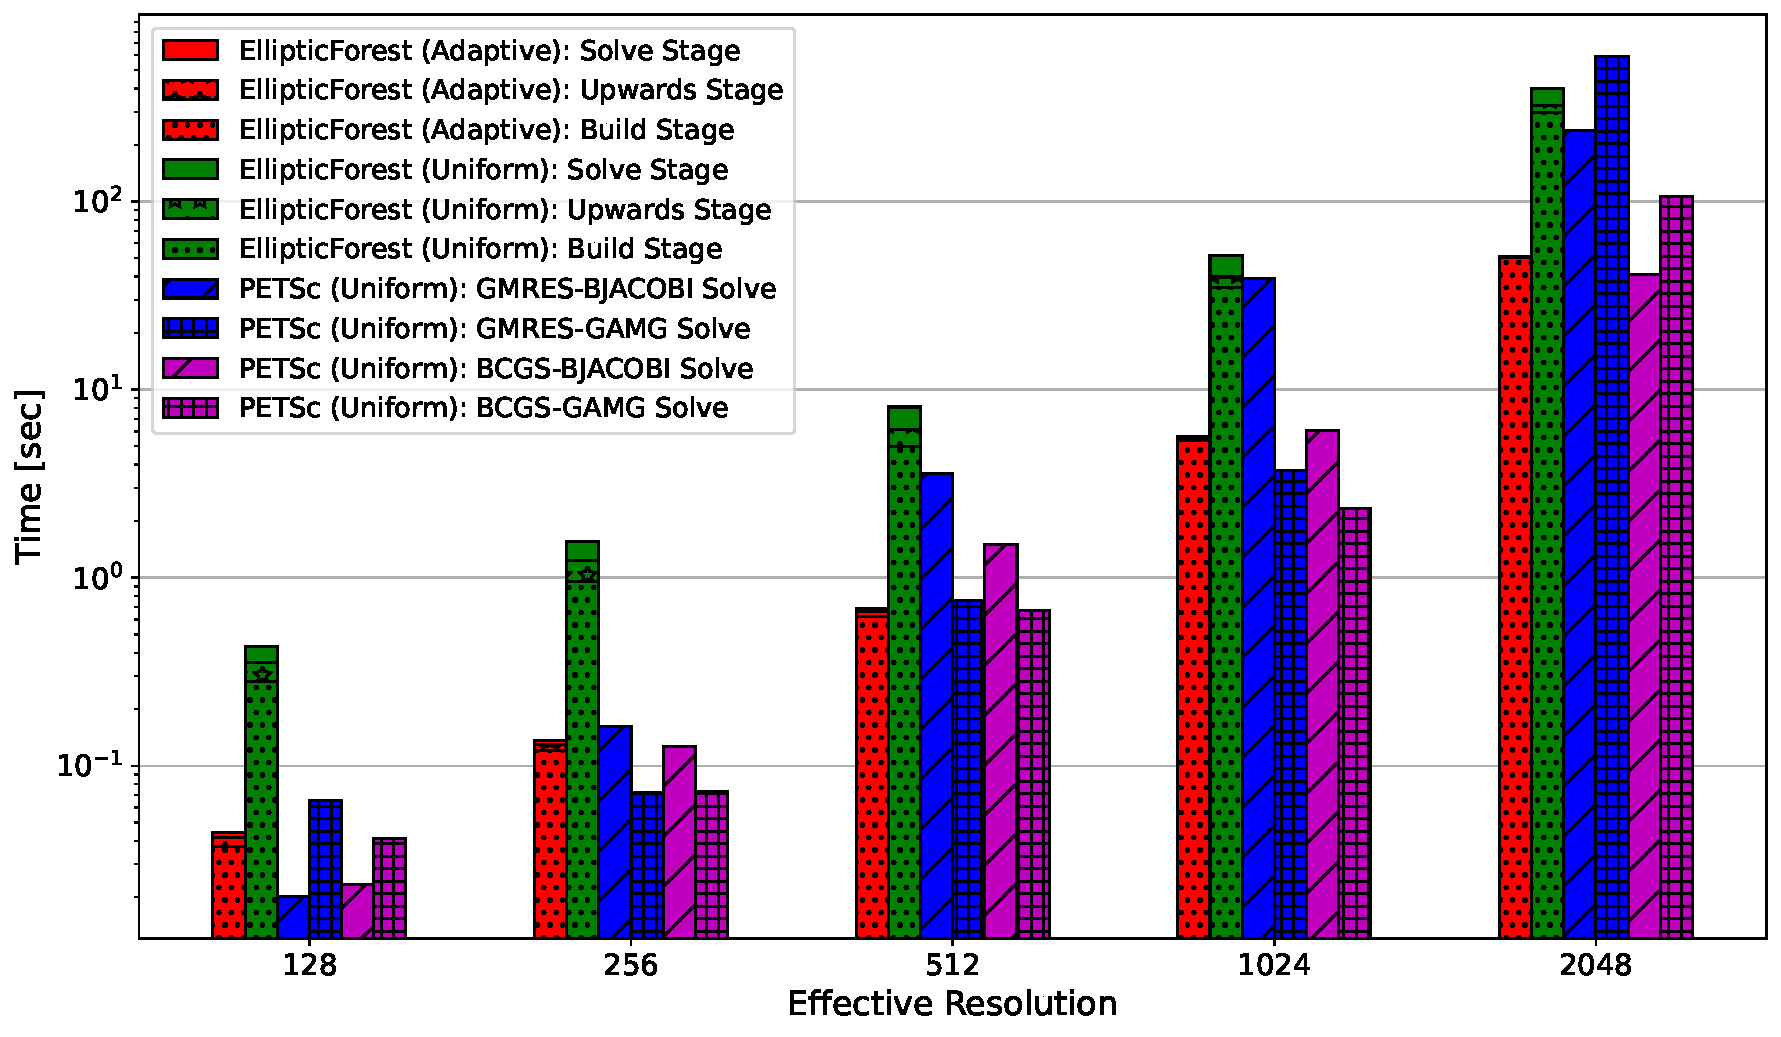
\includegraphics[width=1.0\textwidth, clip=true, trim={0 0 0 0}]{figures/case02-stacked-bar-plot-comparisons-no-title.pdf}
        \caption{Effective resolution vs. timing plots for Case 2 (\refsec{sub:case2}). The effective resolution is the number of cells per side if the mesh were refined to $L_{\text{max}}$. Each color indicates a different method/solver. Patterns indicate different stages or preconditioners. Lower is better.}
        \label{fig:case02-stacked-bar-plot}
    \end{figure}
% \end{landscape}

\begin{figure}
    \centering
    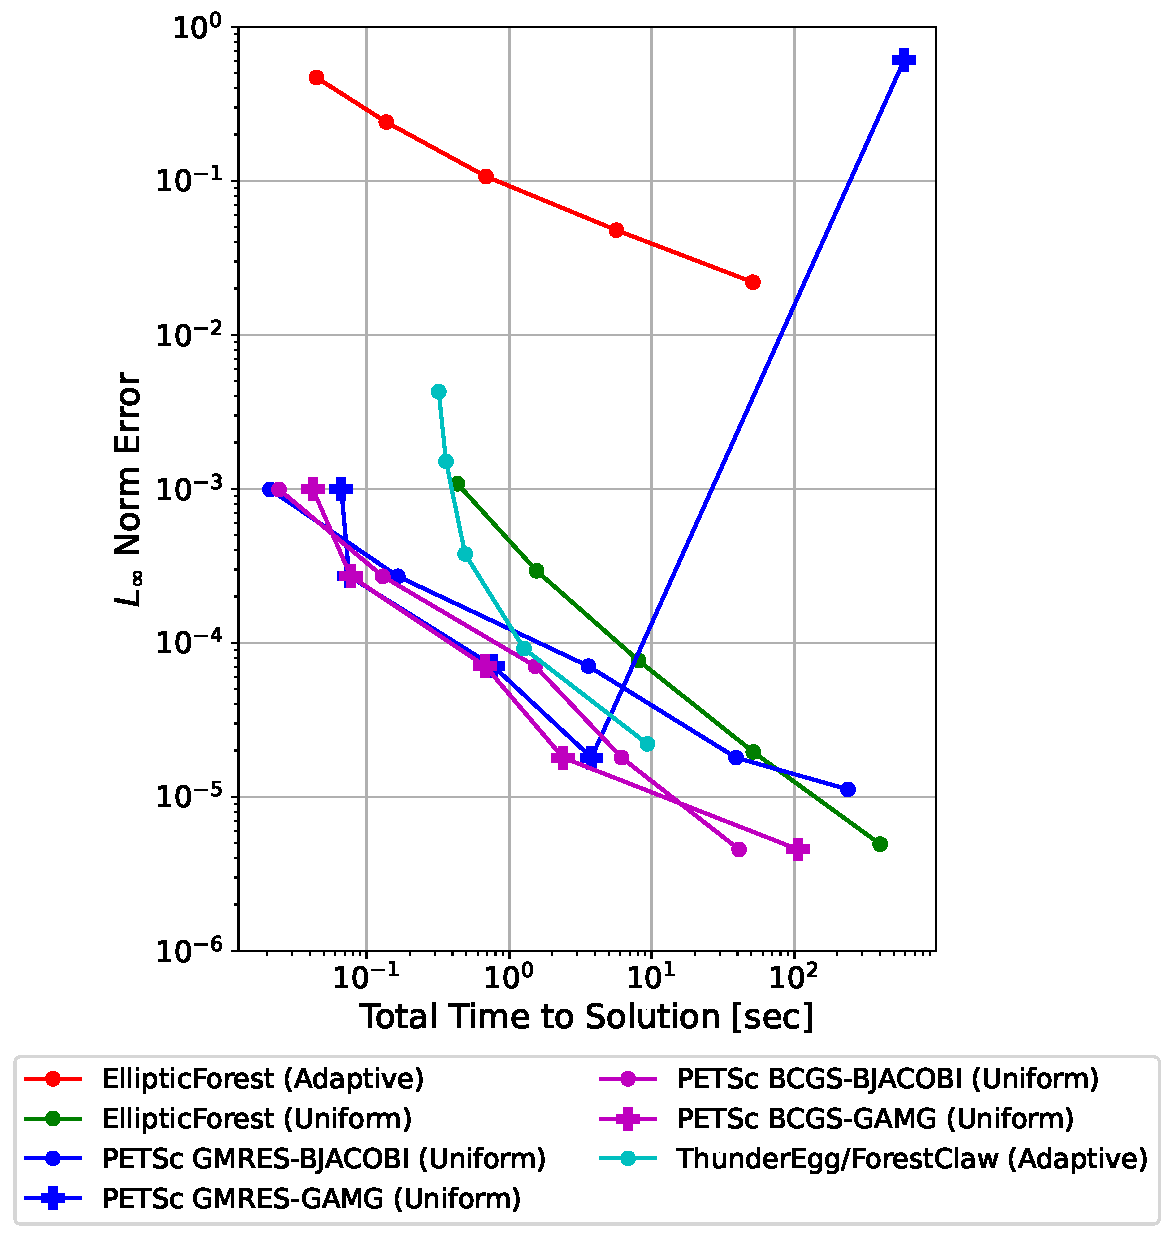
\includegraphics[width=1.0\textwidth, clip=true, trim={0 0 0 0}]{figures/case02-work-precision-plots-no-title.pdf}
    \caption{Work-precision plots for Case 2 (\refsec{sub:case2}). Colors indicate different methods and solvers, while markers indicate the type of preconditioner for certain iterative solvers. Curves that jump to the upper-right region of the plot usually indicate a failure to converge. For work-precision plots, curves that lie in the lower-left portion of the plot are better.}
    \label{fig:case02-work-precision-plot}
\end{figure}

{\bf Discussion}
As a variable coefficient problem, the optimizations we took for the \gls{qahps} method in Case 1 do not apply (operator caching, constructing the \gls{d2n} matrix, and the use of FISHPACK). For iterative solvers, conjugate gradient methods can still be used when $\beta(\textbf{x}) > 0$, as this still leads to a SPD matrix with our finite difference discretization.

Timing results for this case are shown in the stacked bar plot of \reffig{fig:case02-stacked-bar-plot}, similarly to that of Case 1. For all effective resolutions, PETSc's \gls{cg} solvers and \gls{amg} preconditioned \gls{gmres} are the fastest. Uniform \gls{qahps} is the slowest for all effective resolutions, nearly an order of magnitude slower than most other methods. Adaptive \gls{qahps} performs slightly better and is competitive with other solvers at all effective resolutions. ThunderEgg's adaptive solver solves \refeqn{eq:case02-variable-poisson} at the same order of magnitude than PETSc's fastest solvers. As in Case 1, the uniform and adaptive \gls{qahps} reported times include all stages. Subsequent solves need only call the upwards and solve stages, which remain 2-4 orders of magnitude faster than any other method.

As shown in \reffig{fig:case02-work-precision-plot}, all methods show accurate convergence. Most PETSc solvers and uniform \gls{qahps}, solve to the same accuracy measured in the $L_{\infty}$ norm. Block Jacobi preconditioned \gls{gmres} fails to converge at the highest effective resolution. The adaptive \gls{qahps} curve and the adaptive ThunderEgg curve indicates that while the solution does converge, perhaps the mesh refinement criteria did not match regions of error as best as possible.

\subsection{Case 3: The High Wave Number Helmholtz Equation}
\label{sub:case3}

The final case study solves a Helmholtz equation with varying wave number:
\begin{align}
    \nabla^2 u(x,y) + \lambda u(x,y) = 0,
\end{align}
with $(x,y) \in \Omega = [-1, 1]^2$. We vary $\lambda$ according to $[1, 10, 100, 1000]$ to test the various solvers for convergence for wave-like systems with high wave numbers. The wave number $\kappa$ is related to $\lambda$: $\kappa = \sqrt{\lambda}$. The exact solution is that of a wave source located at $(-2, 2)$ with an exact solution of
\begin{align}
    u(x,y) = Y_0(\kappa \sqrt{(x_0 - x)^2 + (y_0 - y)^2}).
\end{align}
The Dirichlet boundary conditions are prescribed using the exact solution. As the solution is highly oscillatory throughout the domain, no adaptivity is used in this case. Rather, this case study is used to compare the performance of direct and iterative solvers for high wave number problems.

For PETSc, we use the GMRES and \gls{bcgs} methods for iterative solvers. The system formed with this discretization is not SPD and thus the \gls{cg} method cannot be used.

\begin{figure}
    \centering
    \begin{subfigure}[t]{0.48\textwidth}
        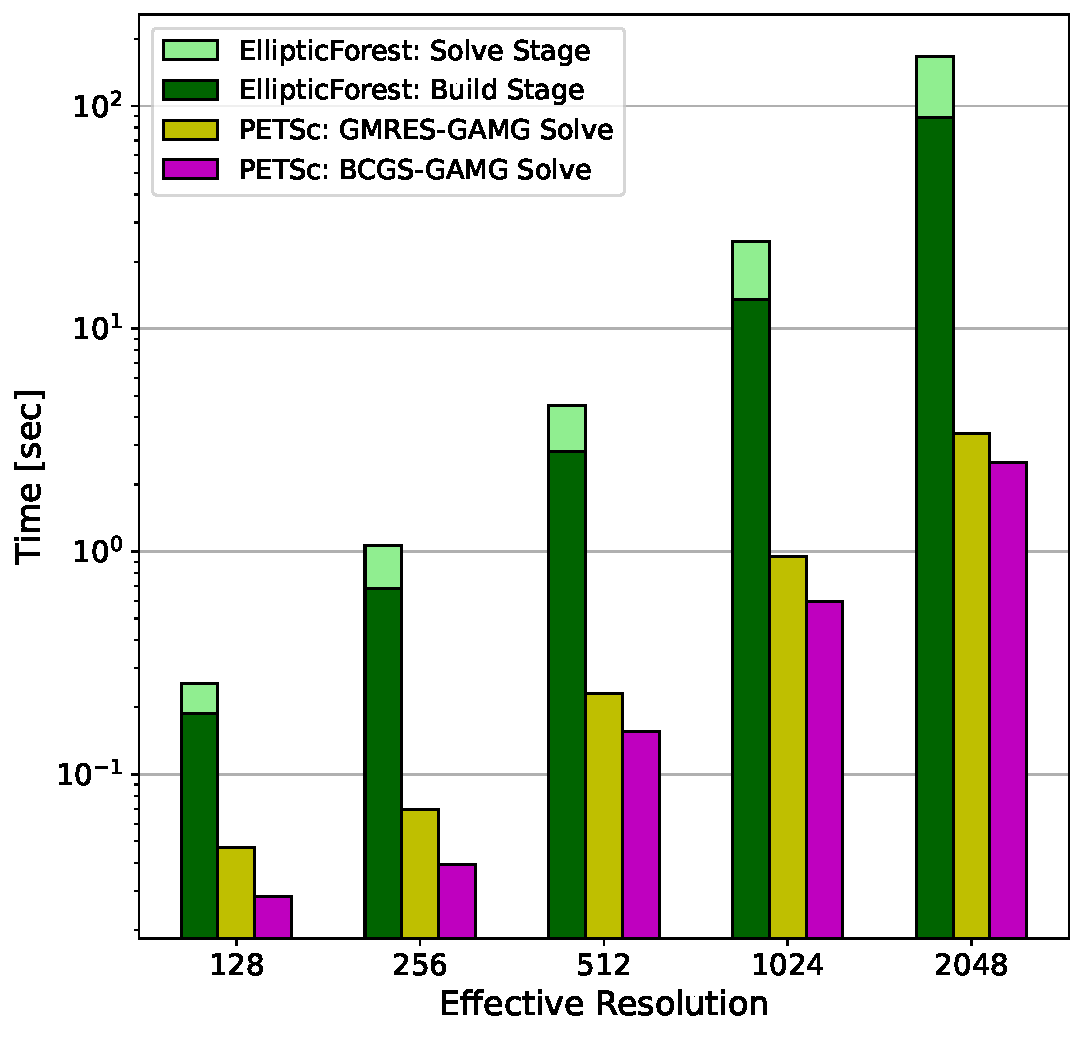
\includegraphics[width=1\textwidth, clip=true, trim={0 0 0 0}]{figures/case03-l1-stacked-bar-plot-comparisons-no-title.pdf}
        \caption{$\lambda = 1$}
    \end{subfigure}
    \begin{subfigure}[t]{0.48\textwidth}
        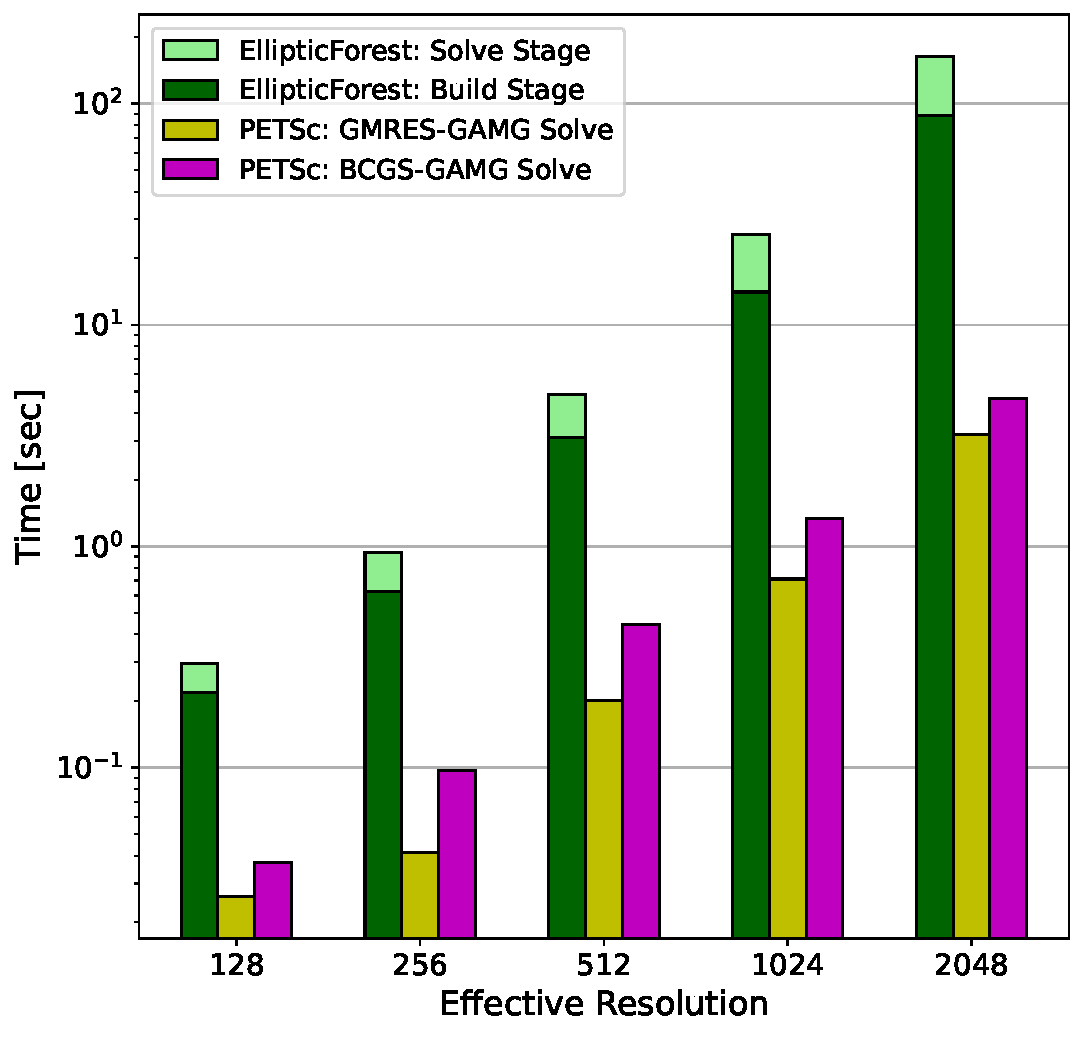
\includegraphics[width=1\textwidth, clip=true, trim={0 0 0 0}]{figures/case03-l10-stacked-bar-plot-comparisons-no-title.pdf}
        \caption{$\lambda = 10$}
    \end{subfigure}
    \begin{subfigure}[t]{0.48\textwidth}
        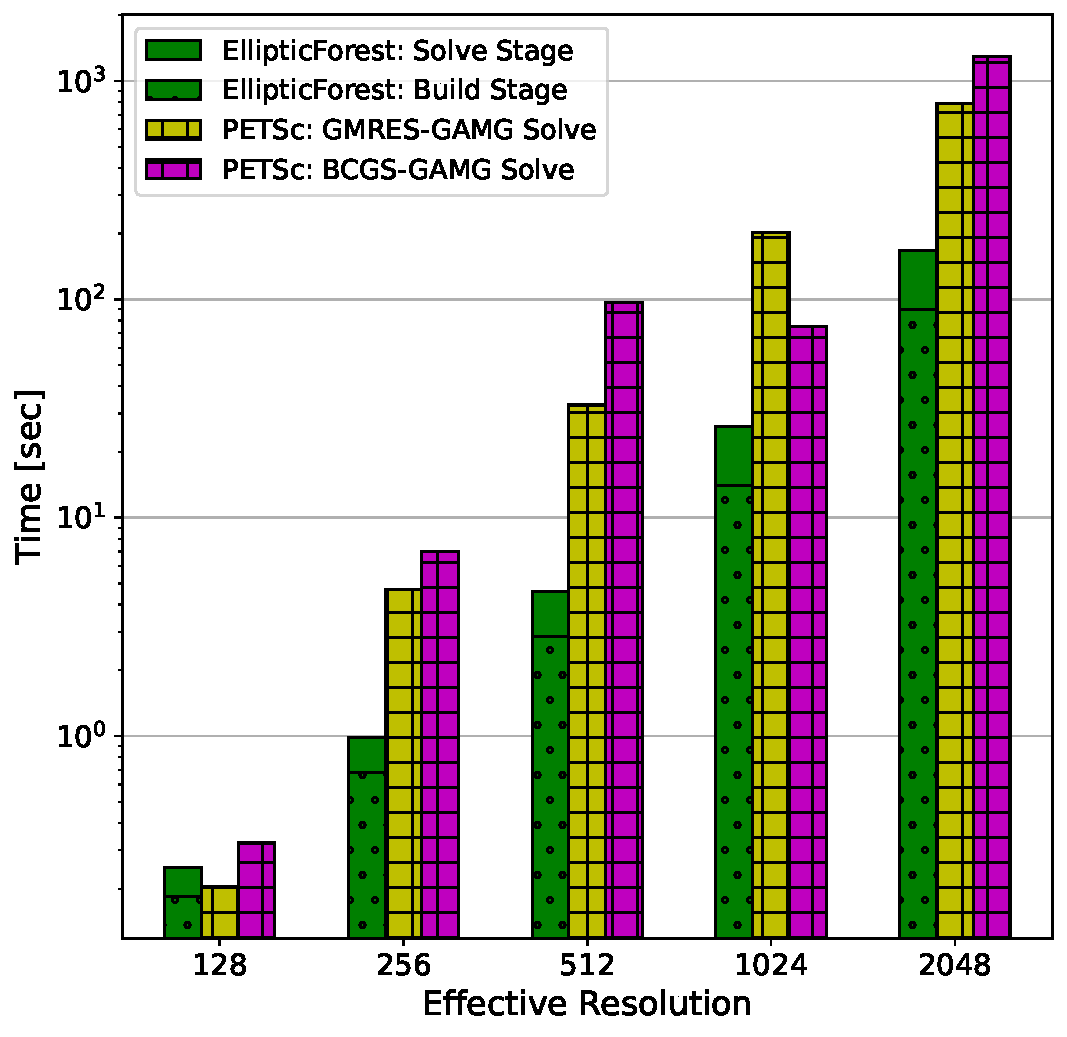
\includegraphics[width=1\textwidth, clip=true, trim={0 0 0 0}]{figures/case03-l100-stacked-bar-plot-comparisons-no-title.pdf}
        \caption{$\lambda = 100$}
    \end{subfigure}
    \begin{subfigure}[t]{0.48\textwidth}
        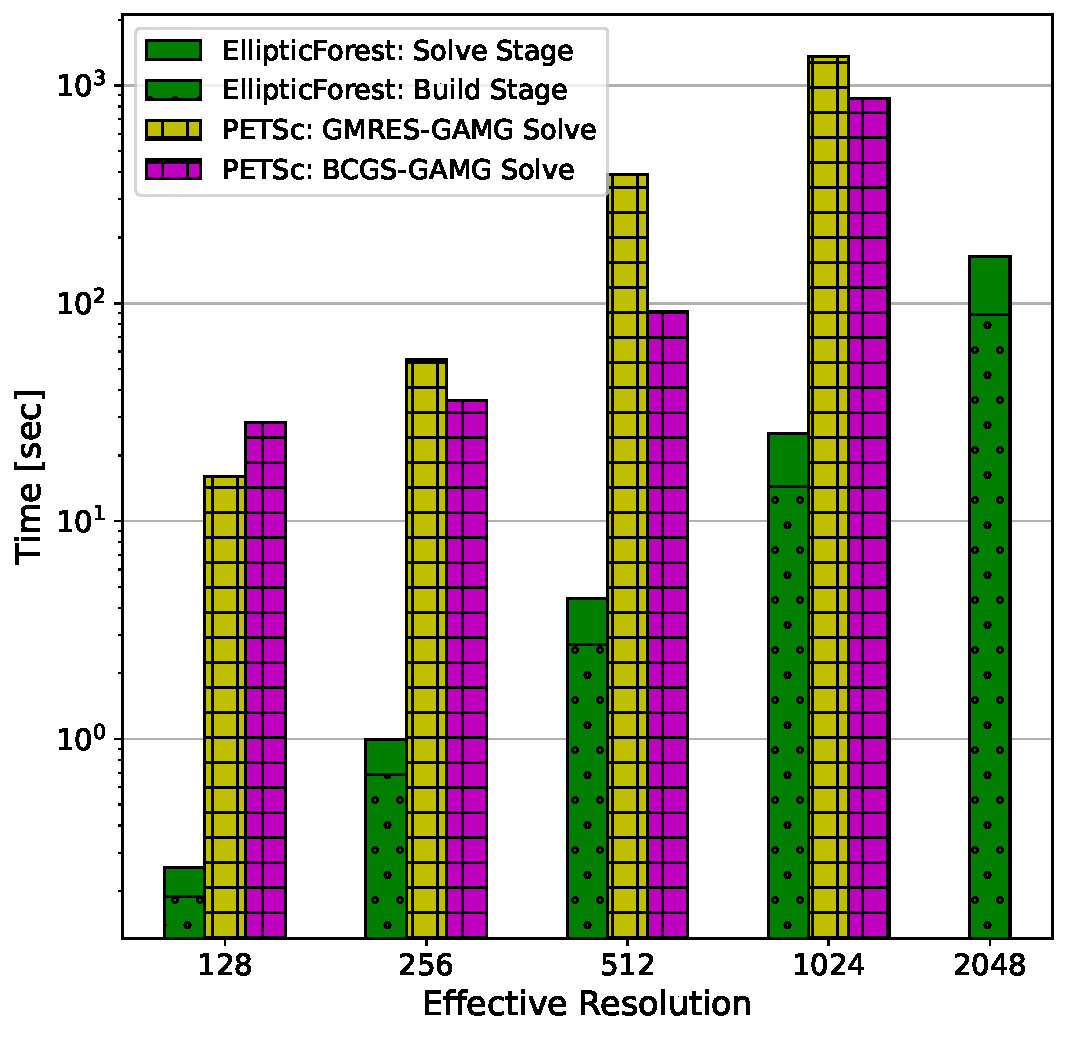
\includegraphics[width=1\textwidth, clip=true, trim={0 0 0 0}]{figures/case03-l1000-stacked-bar-plot-comparisons-no-title.pdf}
        \caption{$\lambda = 1000$}
    \end{subfigure}
    \caption{Effective resolution vs. timing plots for Case 3 (\refsec{sub:case3}). The effective resolution is the number of cells per side. Each color indicates a different method/solver. Patterns indicate different stages or preconditioners. Each plot shows the performance for the solvers at varying $\lambda$. Lower is better.}
    \label{fig:case03-stacked-bar-plot}
\end{figure}

\begin{figure}
    \centering
    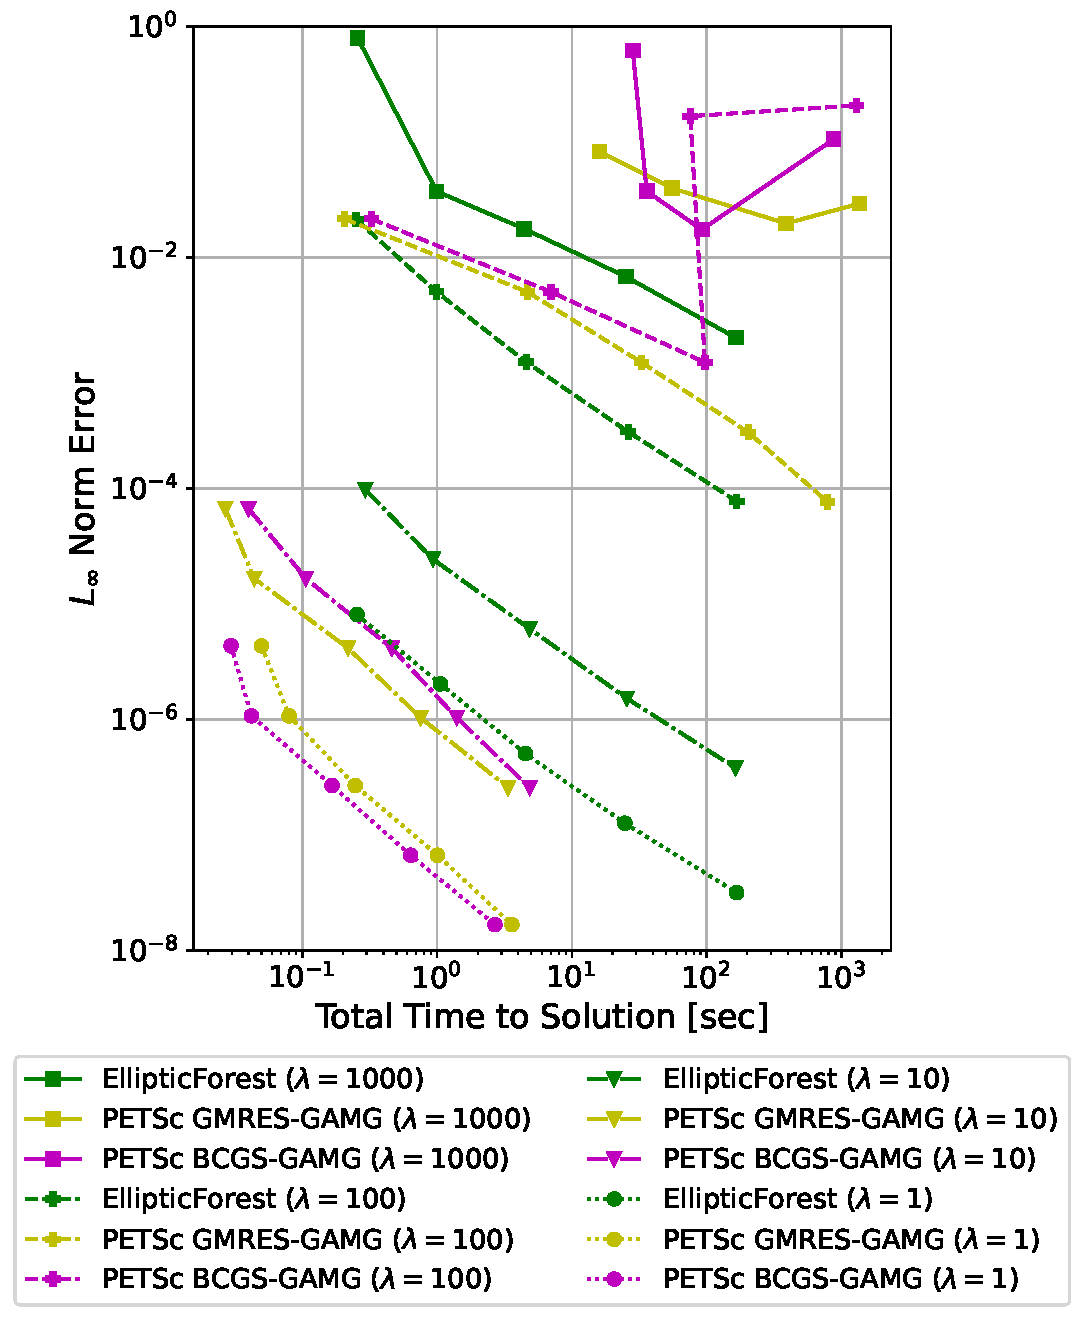
\includegraphics[width=1.0\textwidth, clip=true, trim={0 0 0 0}]{figures/case03-work-precision-plots-no-title.pdf}
    \caption{Work-precision plots for Case 3 (\refsec{sub:case3}). Colors indicate different methods, while markers indicate the value of $\lambda$. Curves that jump to the upper-right region of the plot usually indicate a failure to converge. For work-precision plots, curves that lie in the lower-left portion of the plot are better.}
    \label{fig:case03-work-precision-plot}
\end{figure}

{\bf Discussion}
High wave number problems are notoriously difficult for iterative solvers to converge. Because of this, only \gls{amg} preconditioned PETSc solvers are used as those preconditioned with block Jacobi failed to converge. Direct solvers are often preferred in these applications because they solve the system to machine precision, dependent on the resolution and conditioning of the system matrix. As this is a homogeneous elliptic \gls{pde}, the upwards stage does not need to be called.

\reffig{fig:case03-stacked-bar-plot} shows the effective resolution vs. time to solution for varying $\lambda$. At lower $\lambda$ ($1$ and $10$), both iterative solvers are faster than uniform \gls{qahps}. However, at $\lambda = 100$ and $\lambda = 1000$, uniform \gls{qahps} is faster in nearly all cases. Both iterative solvers struggle to converge, stopping prematurely when the maximum number of iterations is reached. This is more obvious in the work-precision plot \reffig{fig:case03-work-precision-plot}. Both iterative solvers were paused at $R_{\text{eff}} = 2048$ and $\lambda = 1000$ after nearly an hour each.

The work-precision plot found in \reffig{fig:case03-work-precision-plot} indicates that the iterative solvers failed to accurately converge at high $\lambda$. Indeed, the higher error and time to solution of the \gls{gmres} and \gls{bcgs} for $\lambda = 100, 1000$ show this. Uniform \gls{qahps} still manages to converge to the exact solution, albeit slower at higher $\lambda$. The direct solver results suggest that it will continue to converge at higher resolutions. Contrast this to the iterative solvers that would likely fail to converge at all.